\section{node Struct Reference}
\label{structnode}\index{node@{node}}
{\tt \#include $<$bbtracker.h$>$}

Collaboration diagram for node:\nopagebreak
\begin{figure}[H]
\begin{center}
\leavevmode
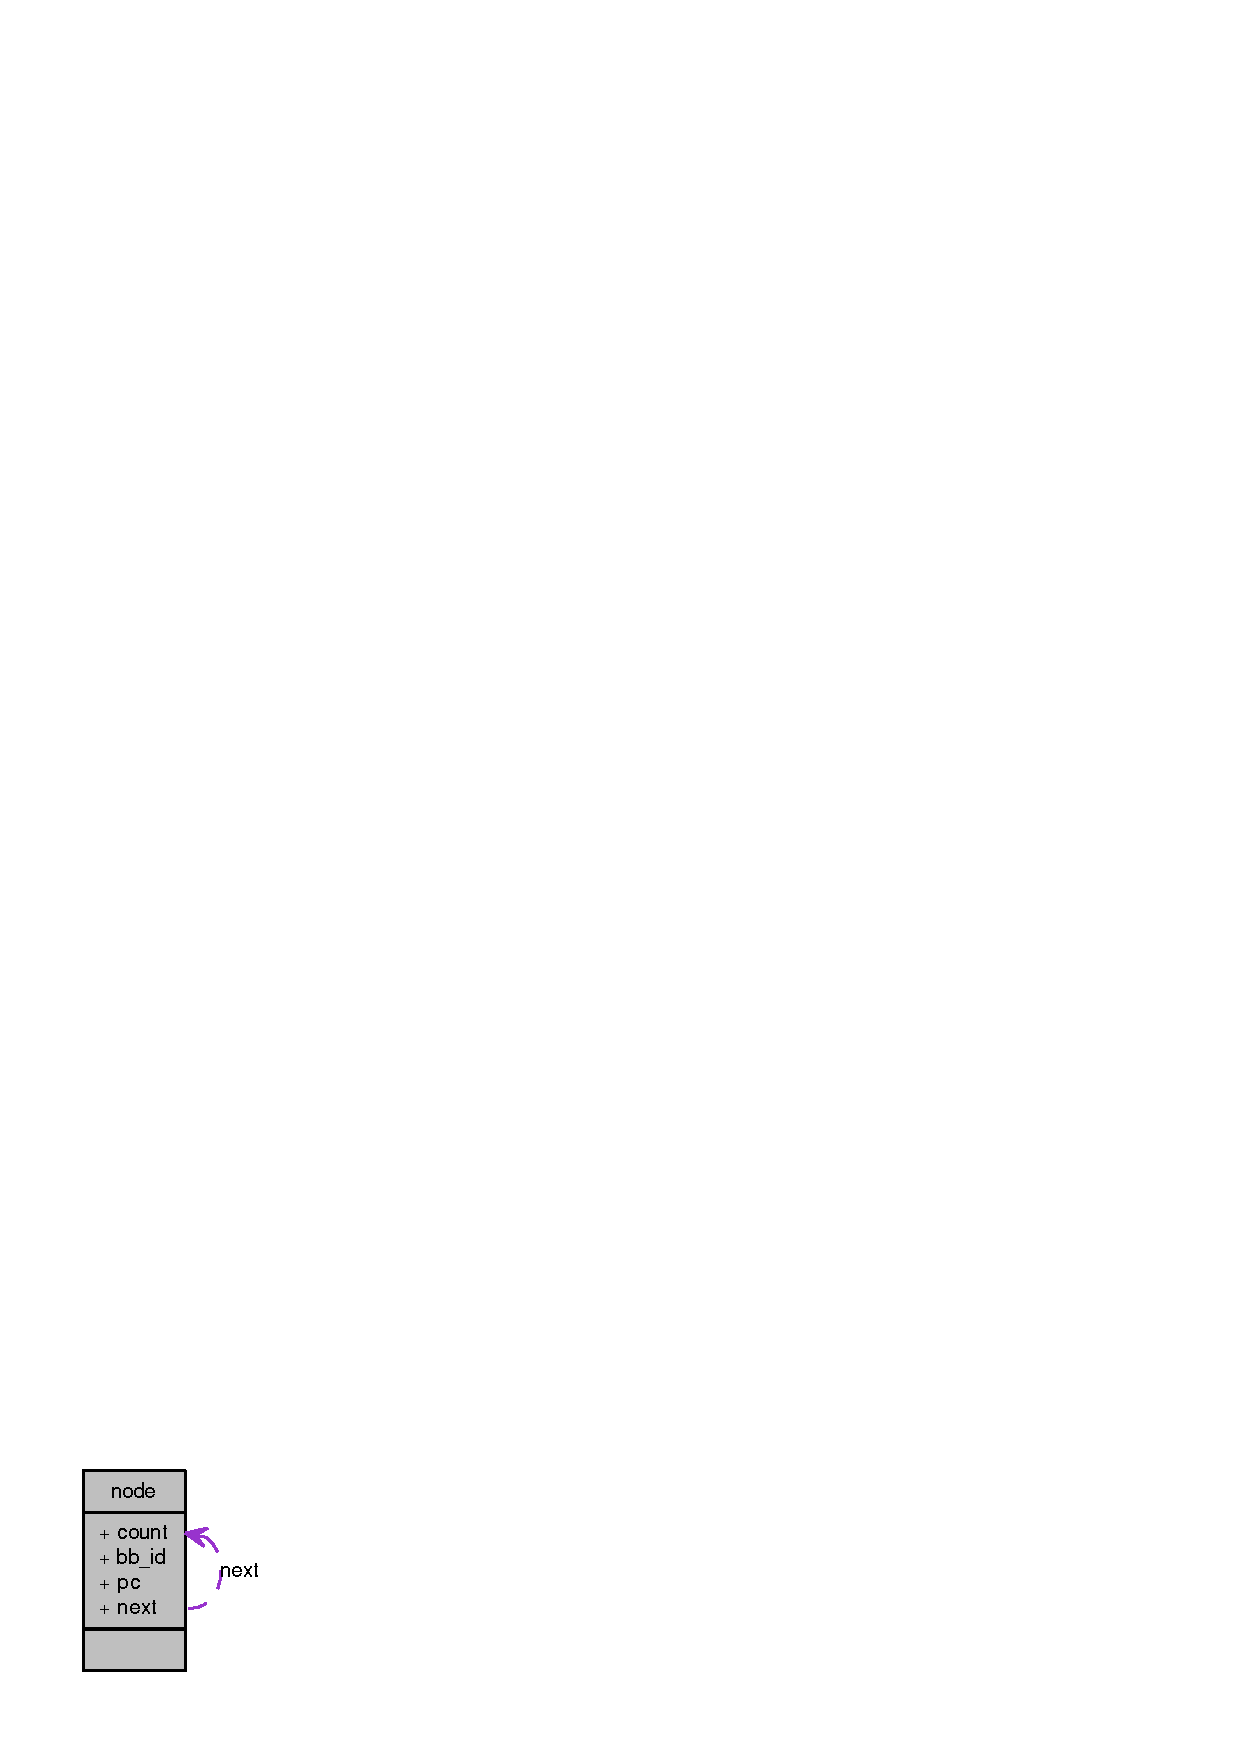
\includegraphics[width=129pt]{structnode__coll__graph}
\end{center}
\end{figure}
\subsection*{Public Attributes}
\begin{CompactItemize}
\item 
int {\bf count}
\item 
int {\bf bb\_\-id}
\item 
long {\bf pc}
\item 
struct {\bf node} $\ast$ {\bf next}
\end{CompactItemize}


\subsection{Detailed Description}


Definition at line 85 of file bbtracker.h.

\subsection{Member Data Documentation}
\index{node@{node}!bb\_\-id@{bb\_\-id}}
\index{bb\_\-id@{bb\_\-id}!node@{node}}
\subsubsection[{bb\_\-id}]{\setlength{\rightskip}{0pt plus 5cm}int {\bf node::bb\_\-id}}\label{structnode_f8b174bf25144314c1caa4728ddb5013}




Definition at line 87 of file bbtracker.h.\index{node@{node}!count@{count}}
\index{count@{count}!node@{node}}
\subsubsection[{count}]{\setlength{\rightskip}{0pt plus 5cm}int {\bf node::count}}\label{structnode_e00bf56112dc8c807b99232c21fadbdc}




Definition at line 86 of file bbtracker.h.\index{node@{node}!next@{next}}
\index{next@{next}!node@{node}}
\subsubsection[{next}]{\setlength{\rightskip}{0pt plus 5cm}struct {\bf node}$\ast$ {\bf node::next}\hspace{0.3cm}{\tt  [read]}}\label{structnode_a3e8aa83f864292b5a01210f4453fcc0}




Definition at line 89 of file bbtracker.h.\index{node@{node}!pc@{pc}}
\index{pc@{pc}!node@{node}}
\subsubsection[{pc}]{\setlength{\rightskip}{0pt plus 5cm}long {\bf node::pc}}\label{structnode_f27f1671794da0670c1d782677a86916}




Definition at line 88 of file bbtracker.h.

The documentation for this struct was generated from the following file:\begin{CompactItemize}
\item 
{\bf bbtracker.h}\end{CompactItemize}
